\section{Ensemble methods}
The problem with \textit{decision trees} is their instability on the training data: small chnages in the training dataset might lead to noticeable changes in the prediction.\\
\begin{figure}[h]
    \centering
    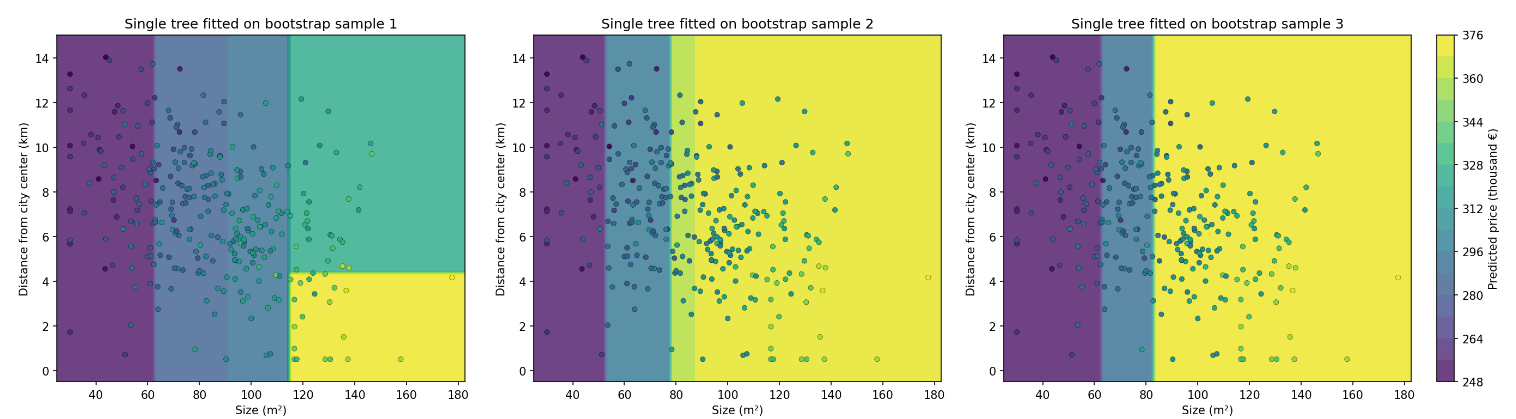
\includegraphics[width=0.8\linewidth]{img//tree-models/dectree_inst_example.png}
\end{figure}
To address this we can shift to \textbf{ensemble methods} := collection of models whose prediction are combined. These models $\hat{f}_1(x)...\hat{f}_B(x)$ might differ under several aspects: they may use different algorithms, different hyperparameters, different samples ... and if these models make different errors, combining them might cancel out part of it: \textbf{a combination of not-identical and not-perfectly correlated models may lead to a more stable prediction}.\\
$$
\hat{f}_{\text{ens}}(x) = \frac{1}{B} \sum_{b=1}^{B} f_b(x)
$$
If the models are independent and have the same variance $\mathbb{V}[\hat{f}_b(x)]=\sigma^2$ then:\\
$$
\text{Var}(\hat{f}_{\text{ens}}(x)) = \text{Var}\left(\frac{1}{B}\sum_{b=1}^{B} f_b(x)\right) = \frac{1}{B^2}\sum_{b=1}^{B} \text{Var}(f_b(x)) = \frac{1}{B^2} B\sigma^2 = \frac{\sigma^2}{B}
$$
however in practise these models are not independent (often they use the same predictors), instead they have some degree of \textit{pairwise correlation} $\rho$, ending up with something similar to the ideal case:\\
$$
\text{Var}(\hat{f}_{\text{ens}}(x)) = \rho\sigma^2 + \frac{1-\rho}{B}\sigma^2
$$
for $B\to\infty$ we get that $\mathbb{V}[\hat{f}_{ens(x)}]\to\rho\sigma^2$, meaning that the outcomme is better when individual models are not too correlated.\\
\vspace{0.2cm}

\textcolor{green!60!black}{\textbf{Pros:}}
\begin{itemize}
    \item \textbf{computational scalability}: when the dataset is too large, we can split the dataset and train a model on different partitions (divide-et-impera)
    \item \textbf{robustness to sample variablity}: if data instead is limited, we can take different resamples trying to obtain different models, reducing the overhall instability
    \item \textbf{complementary views combination}: we can let different models tackle different aspects of the data (like one model for linear trends, one for interactions ...)
\end{itemize}
\vspace{0.2cm}
The question now is, how do we create diversity in an ensemble in order to have as much independency as possible?

% -------------------------------------------------------------------------------------------------------------
\newpage
\subsection{Bootstrapping and AGGregaING (BAGGING)}
The idea is to train several models on different sample of data, using for example bootstraping, turning unstable trees into a more stable model by averaging them.
$$
D^{*1}...D^{*B} \quad\to \hat{f}^{*1}(x)...\hat{f}^{*B}(x) \quad\to \hat{f}_{BAG}(x)=\frac{1}{B}\sum_{b=1}^B\hat{f}^{*b}(s)
$$
\begin{figure}[h]
    \centering
    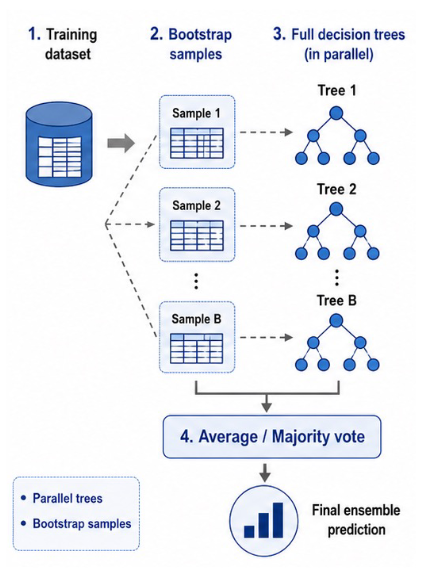
\includegraphics[width=0.3\linewidth]{img//tree-models//bagging/bagging_concept.png}
\end{figure}

\subsubsection{Bagging evaluation}
As seen before we have that with bootstraping 36.8\% of the datapoints are left out by each boostrap sample, why not use them to test the model without creating a test set?\\
Each tree has been trained using the boostrap sample $D^{*b}$, we have the \textbf{out-of-bag (OOB) set $\mathcal{B_{- i}=\{b_i\notin D^{*b}\}}$} composed of the observations never used for any tree training. We test our model on this new dataset.
$$
\hat{f}_{OOB}(x_i)=\cfrac{1}{|\mathcal{B}_{-i}|}\sum_{b\in\mathcal{B}_{-i}}\hat{f}_b(x_i) \to \text{OOB MSE}=\frac{1}{n}\sum_{i=1}^n\left(y_i-\hat{f}_{OOB}(x_i)\right)^2
$$
\begin{figure}
    \centering
    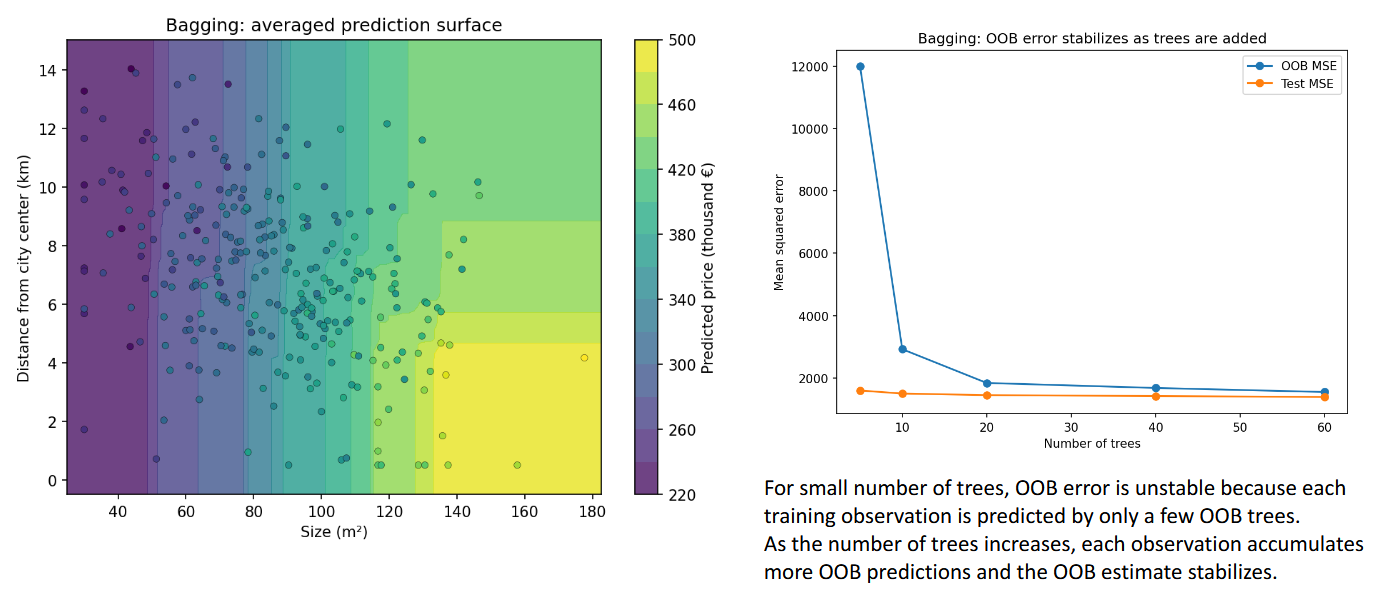
\includegraphics[width=0.8\linewidth]{img//tree-models//bagging/bagging_oob.png}
\end{figure}

\subsubsection{Bagging tree depth}
How in depth should Bagging tree grow? A deeper tree has low bias but high variance, which is leveraged by bagging \arrow build many trees to obtain low bias, meaning deep trees, and let Bagging manage the variance 

\subsubsection{Applicability}
Baggin make sense only if the data has high varianca by itself, otherwise is useless applying Baggin to leverage a non-existent variance.\\
\vspace{0.2cm}
\textcolor{green!60!black}{\textbf{Examples where bagging helps:}}
\begin{itemize}
    \item decision trees
    \item high-flexibility models
    \item unstable model-selection procedures and base learner unstable
\end{itemize}

\textcolor{red}{\textbf{Examples where bagging helps less:}}
\begin{itemize}
    \item very stable linear models
    \item strongly regularized models
    \item low-variance algorithms
\end{itemize}

Also there is another big limit: if one predictor is very strong many trees will choose it at the top, making them look similar and correlated, reducing the overhall model variance less effectively.

% -------------------------------------------------------------------------------------------------------------
\vspace{0.3cm}
\subsection{Random forest}
The idea is add another source of randomness w.r.t. Bagging: instead of using on each boostrap sample the whole set of predictors, each time take a subset of them \arrow this allows to reduce the correlation between trees forcing them to be more diffent.
$$
D^{*1}...D^{*B} \quad\to \hat{f}_1(x)...\hat{f}_B(x) \text{ on feature subset}\quad\to \hat{f}_{RF}(x)=\frac{1}{B}\sum_{b=1}^B\hat{f}_b(s)
$$
\begin{figure}[h]
    \centering
    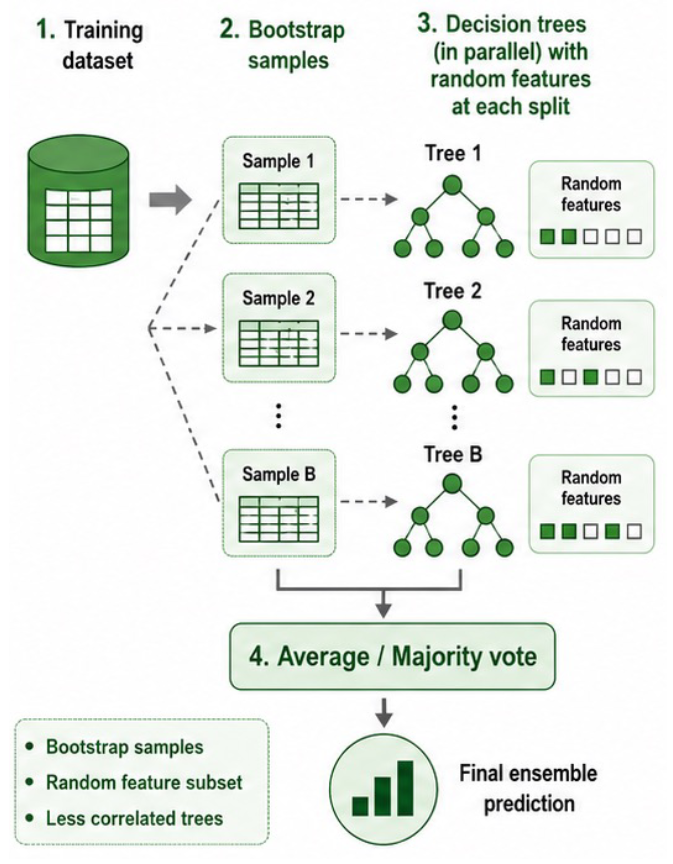
\includegraphics[width=0.3\linewidth]{img//tree-models//bagging/rndforest.png}
\end{figure}
\newpage
We have one more hyperparam: $m$, how many features we use at each split. The smaller the $m$ the more different the trees will be; some "rule of thumb" is to take $m=\sqrt{p}$ for classification and $m=\frac{p}{3}$ for regression. This hyperparam also influencse how many trees we should use: bigger $B$ usually means more stable predictors and rarely causes the model to overfit; good values could be found by trying out several options and choose the value for which the error starts stabilizing.
\begin{figure}[h]
    \centering
    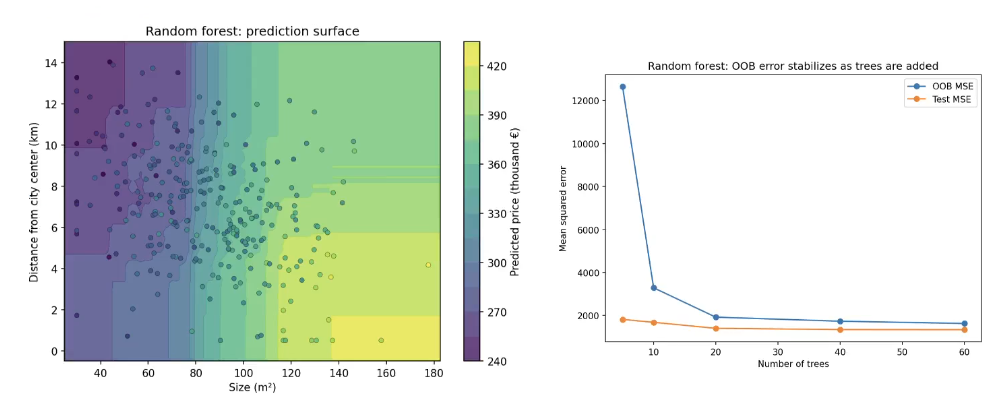
\includegraphics[width=0.9\linewidth]{perf_randforst.png}
\end{figure}

\subsubsection{Feature importance}
Random forest can be used also to exploit the importance of predictors, like some sort of embedded feature selection. There are two main types of importance:
\begin{description}
    \item[impuruty-based importance]: some feature is more important if splitting on it frequently reduces the overhal RSS.
    \item[permutation importance]: based on the idea that on how much the model performance degradate by randomly permute the variable value, the more this deagradation is the more the feature is important.
\end{description}

\begin{figure}[h]
    \centering
    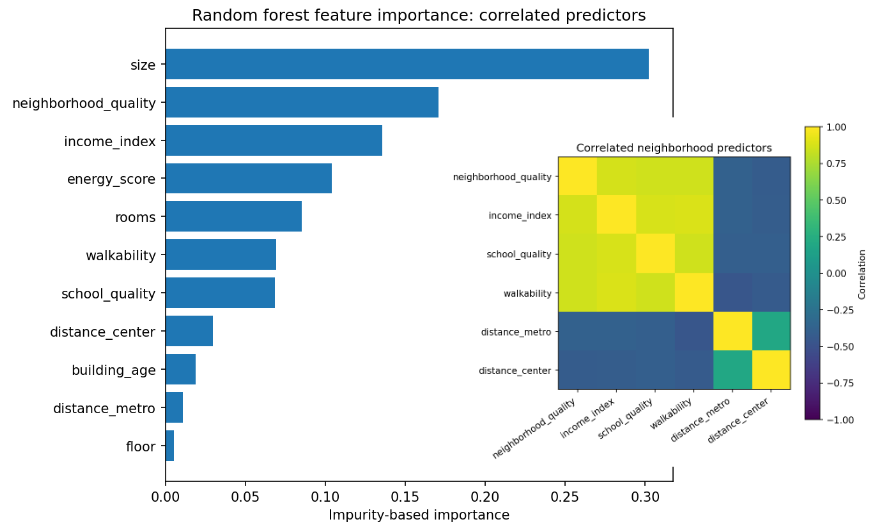
\includegraphics[width=0.5\linewidth]{img//tree-models//randomforest/corr_pred_randfor.png}
\end{figure}
Random forst feature selection might be dangerous when we deal with correlated predictors: importance might be splitted among them and the method might end up using different members on the splits with the same outcome, making individual feature importane smaller and the selection unstable acros different samples.

% -------------------------------------------------------------------------------------------------------------
\newpage
\subsection{Boosting}
The idea is creatin the model sequentially instead that parallely, trying with each new model to improve the previous one by exploiting where it has peformed poorly.
$$
\hat{f}_1\to\hat{f}_2\to...\hat{f}_B\quad\Rightarrow \hat{f}_{boost}(x)=\sum_{b=1}^B\gamma_b\hat{h}_b(x)\quad \text{where $\gamma$ := weight, $\hat{h}_n$ := weak learner}
$$
\begin{figure}[h]
    \centering
    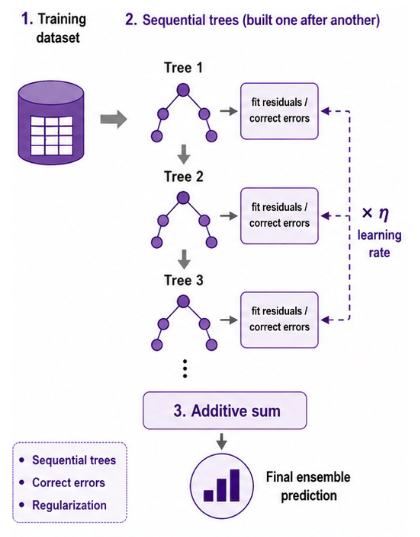
\includegraphics[width=0.3\linewidth]{img//tree-models//boosting/boosting_idea.png}
\end{figure}

It can be seen as building an additive model in which at each step we add a new tree with some learning rate $\eta$ which balance the effect of the new model, and this new tree is fitted in order to reduce the current loss \arrow we use \textbf{gradient boost} to exploit the direction that reduces the loss, and each new weak learner makes a small contribution.
\begin{figure}[h]
    \centering
    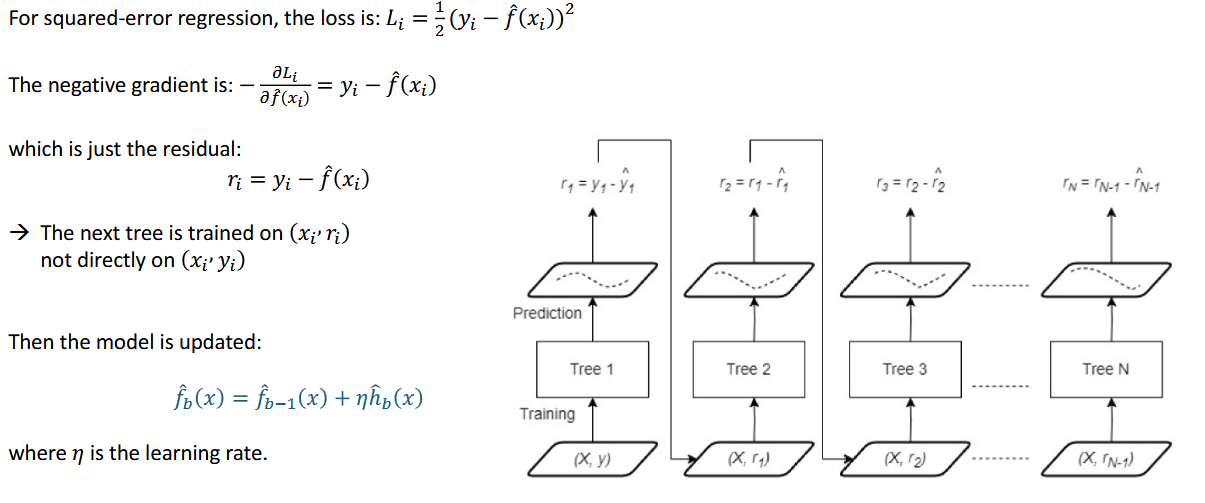
\includegraphics[width=1\linewidth]{img//tree-models//boosting/gradient_boosting.png}
\end{figure}

\newpage
But why do we like to use \textit{weak} learners? They reduce the risk of overfittig, each one of them capturing one simple local structure which together they'll form an approximated complex function.
\begin{figure}[h]
    \centering
    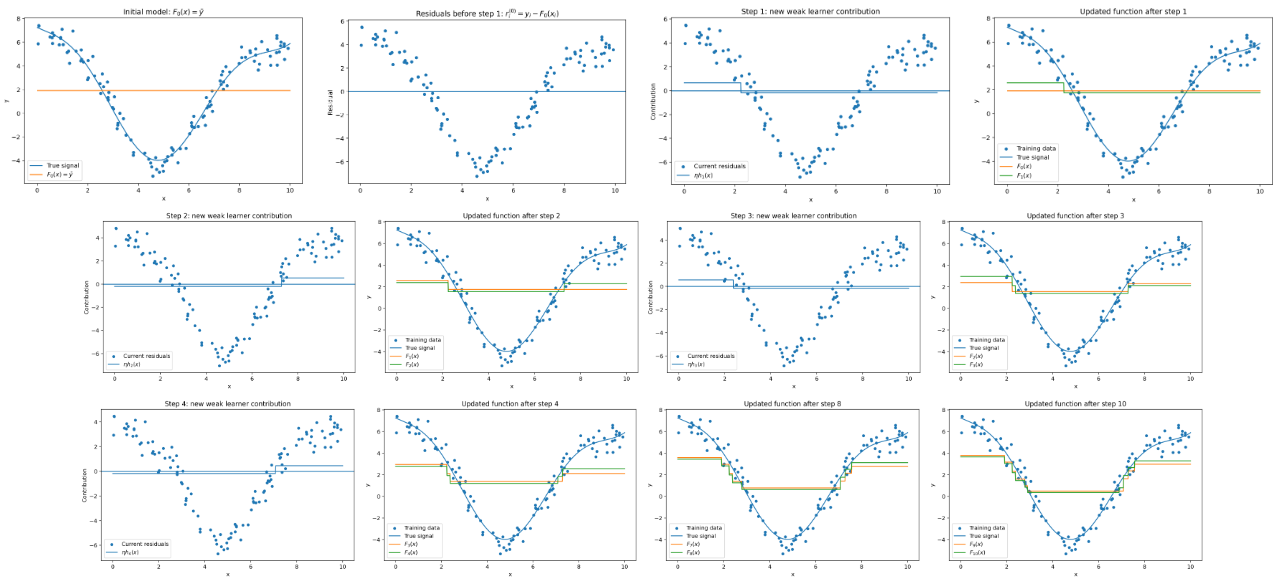
\includegraphics[width=0.95\linewidth]{img//tree-models//boosting/gradient_boost_incr_steps.png}
    \caption*{Basically at each step we add a step function}
\end{figure}
\begin{figure}[h]
    \centering
    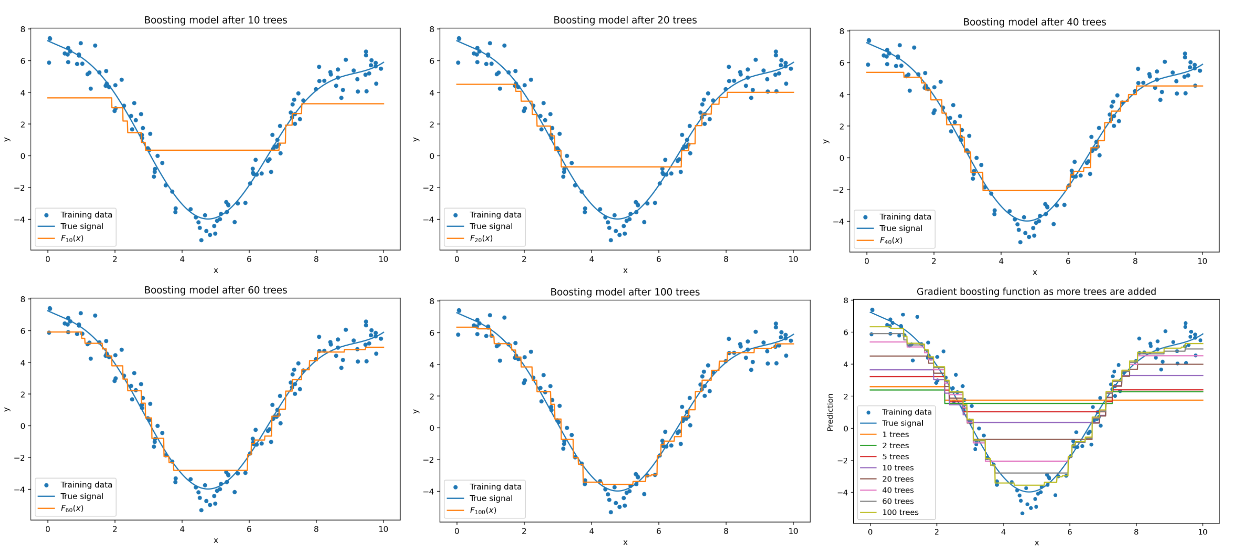
\includegraphics[width=0.8\linewidth]{img//tree-models//boosting/gradient_descend_boosting.png}
\end{figure}

Since boosting methods can easily overfit, we must regularize them by balacing the $B$ := num of trees, $\eta$ and the $\text{tree depth}$ := complexity of the single learner.

\subsubsection{eXtreme Gradient Boosting (XGBoost)}
It's one very optimized variant of boosting framework, actually used in real life; it's designed to be computationally efficient, can find approximate splits, handle sparse data and scale quite good.

First of all is uses a \textbf{regularized objective}:
$$
\mathcal{L} = \sum_{i=1}^{n} \ell(y_i, \hat{y}_i) + \sum_{m=1}^{M} \Omega(h_m)
\quad\text{where }\ 
\Omega(h) = \gamma T + \frac{1}{2}\lambda \sum_{j=1}^{T} w_j^2\quad T\text{ := num of leafs}, w_j\text{ := prediction score of the leaf}
$$

To further boost efficiency:
\begin{itemize}
    \item second-order optimization on the gradient boosting
    \item sampling at weak learner creation, both for the data the new model is trained on and for the feature used
\end{itemize}


% -------------------------------------------------------------------------------------------------------------
\subsection{Stacking}
We can also think of mixing different algorithms together by adding on top of them a \textbf{meta-learner} $g$ which is charge of combining the results. This might be very useful if we merge alorithms with different results.\\
$$
\hat{f}_{stack}(x)=g\left(\hat{f}_1(x),\ \hat{f}_2(x) ...\hat{f}_B(x)\right)
$$
\begin{figure}[h]
    \centering
    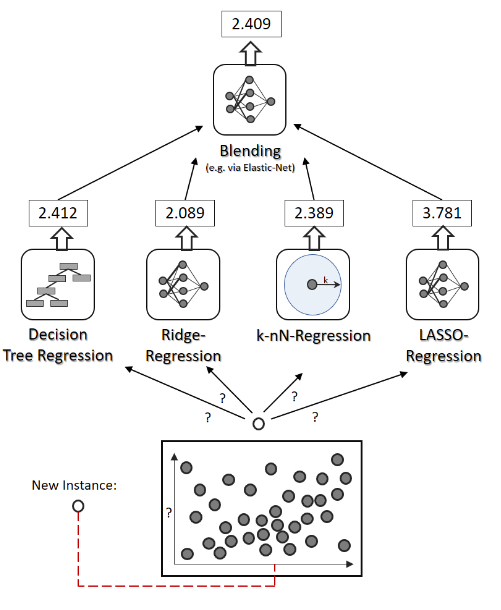
\includegraphics[width=0.5\linewidth]{img//tree-models/stacking.png}
\end{figure}

One simple example is using a lineare model as meta-learner:
$$
\hat{f}_{\text{stack}}(x) = \alpha_0 + \alpha_1 \hat{f}_1(x) + \alpha_2 \hat{f}_2(x) + \cdots + \alpha_B \hat{f}_B(x)
$$
By adjusting the weight of each sub-model the meta-learner chooses the adequate predictor, giving them an implicit importance \arrow the meta-learner learns how to select the right algorithm among those available.
\vspace{0.2cm}
We can see that meta-learners must be trained differently from the models underly them: it must not be trained on predictions made by models on the same observations used to fit them.
\begin{enumerate}
    \item split the data in fold and train/test the base models using cross-validation
    \item collect some observations and make some predictions on them
    \item train the meta-learner on these "out-of-fold" observations
    \item re-fit the base models on the new full dataset
\end{enumerate}